\section*{Assignment 03: Evolution of the Platform Concept}
\addcontentsline{toc}{section}{Assignment 03: Evolution of the Platform Concept}

\subsection*{Where we started}
My first sketches revolved around a ``dinner experiences'' marketplace that matched home chefs with curious guests. It fit the zeitgeist but clashed with why I took the course. Even light desk research and the VirtuAI quick-case debrief \citep{Gunasilan2024} exposed two red flags: regulators already scrutinise informal food businesses, and I had zero logistics advantage. Overlaying \citet{Choudary2016}'s typology made it obvious the idea drifted toward an asset-heavy service, not the orchestrator I wanted to study.

\subsection*{Moments that changed the trajectory}
The pivotal moment came while streaming Lecture~6, when a guest NGO described how hard it is to scope student projects without hand-holding. That story made me revisit my own campus experience and birthed SkillSync: a student--organisation matchmaking platform focused on scoped, time-bound collaborations. I mapped the new interaction using the platform design toolkit from \citet{Reillier2017}, prototyped scoping templates in Figma, and imagined hallway tests with NGOs from previous course projects to stress-test the prompts. Another turning point was analysing monetisation for the home-chef idea. The numbers crumbled under \citet{Porter2008}'s competitive pressure, yet the same analytical exercise illuminated how SkillSync could monetise through completion-based fees and partner enablement. The pivot looks dramatic on paper, but in practice it was a sequence of incremental thought experiments guided by data and theory, echoing the cautionary tales from Lecture~6 about platforms that misread winner-take-all dynamics \citep{Lecture06}. One example of such a thought experiment involved sketching a two-week concierge test where I would manually match a handful of student teams to NGO briefs to validate workflow pain points before investing in automation.

\subsection*{Reflection on the path taken}
Was sticking with SkillSync the optimal play? Mostly yes. The concept matches my comparative advantage (campus networks plus prior student-consulting experience) and gives me a clean cross-side interaction to analyse. I still moved too slowly on validating willingness to pay. If I could rewind the planning phase, I would run pricing conversations alongside prototyping instead of waiting for a polished deck. \citet{HagiuWright2013} warn that deferring business-model validation makes pivots harder later, and I would keep a thinner backlog so sunk-cost bias pops sooner.

Figure~\ref{fig:project-creation} grounds the pivot: the organisation-side wizard forces clarity on outcomes, timelines, support assets, and evaluation criteria with helper text so NGOs feel coached rather than interrogated.

\begin{figure}[H]
  \centering
  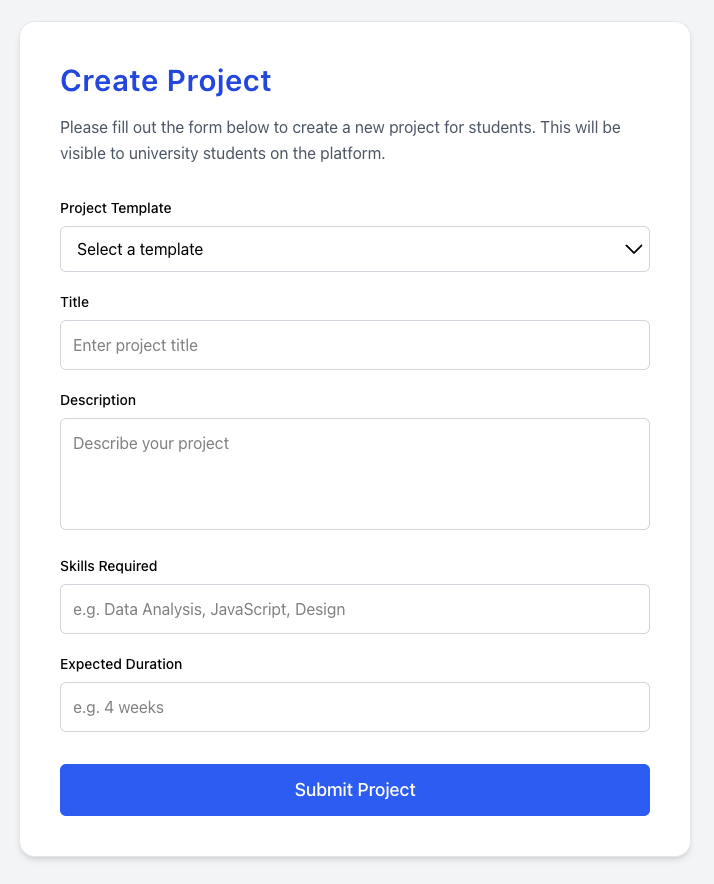
\includegraphics[width=0.85\linewidth]{figures/Organisation-generate-project.png}
  \caption{Organisation project wizard mock-up with scoped-brief guidance.}
  \label{fig:project-creation}
\end{figure}

The expanded scope also let me document decision hygiene. Fortnightly retros --- currently just prompts in my planning doc --- score each experiment on desirability, feasibility, and viability. When the food marketplace keeps ranking low on feasibility the notes justify the pivot, while SkillSync experiments stay attractive thanks to campus networks. The rituals aim to operationalise \citet{Choudary2016}'s iterative governance and \citet{Srnicek2017}'s legitimacy checks once a team spins up.
